\PassOptionsToPackage{usenames,fixpdftex,dvipsnames,svgnames,x11names}{xcolor}
\PassOptionsToPackage{hyphens}{url}
\PassOptionsToPackage{font=small,labelfont=bf,labelsep=period,justification=RaggedRight,format=plain}{caption}

\documentclass[
  oneside,
  openany,
  numbers=noendperiod,
  parskip=half,
  bibliography=totoc
]{scrbook}\usepackage[]{graphicx}\usepackage{xcolor}
%% maxwidth is the original width if it is less than linewidth
%% otherwise use linewidth (to make sure the graphics do not exceed the margin)
\makeatletter
\def\maxwidth{ %
  \ifdim\Gin@nat@width>\linewidth
    \linewidth
  \else
    \Gin@nat@width
  \fi
}
\makeatother

\definecolor{fgcolor}{rgb}{0.345, 0.345, 0.345}
\newcommand{\hlnum}[1]{\textcolor[rgb]{0.686,0.059,0.569}{#1}}%
\newcommand{\hlstr}[1]{\textcolor[rgb]{0.192,0.494,0.8}{#1}}%
\newcommand{\hlcom}[1]{\textcolor[rgb]{0.678,0.584,0.686}{\textit{#1}}}%
\newcommand{\hlopt}[1]{\textcolor[rgb]{0,0,0}{#1}}%
\newcommand{\hlstd}[1]{\textcolor[rgb]{0.345,0.345,0.345}{#1}}%
\newcommand{\hlkwa}[1]{\textcolor[rgb]{0.161,0.373,0.58}{\textbf{#1}}}%
\newcommand{\hlkwb}[1]{\textcolor[rgb]{0.69,0.353,0.396}{#1}}%
\newcommand{\hlkwc}[1]{\textcolor[rgb]{0.333,0.667,0.333}{#1}}%
\newcommand{\hlkwd}[1]{\textcolor[rgb]{0.737,0.353,0.396}{\textbf{#1}}}%
\let\hlipl\hlkwb

\usepackage{framed}
\makeatletter
\newenvironment{kframe}{%
 \def\at@end@of@kframe{}%
 \ifinner\ifhmode%
  \def\at@end@of@kframe{\end{minipage}}%
  \begin{minipage}{\columnwidth}%
 \fi\fi%
 \def\FrameCommand##1{\hskip\@totalleftmargin \hskip-\fboxsep
 \colorbox{shadecolor}{##1}\hskip-\fboxsep
     % There is no \\@totalrightmargin, so:
     \hskip-\linewidth \hskip-\@totalleftmargin \hskip\columnwidth}%
 \MakeFramed {\advance\hsize-\width
   \@totalleftmargin\z@ \linewidth\hsize
   \@setminipage}}%
 {\par\unskip\endMakeFramed%
 \at@end@of@kframe}
\makeatother

\definecolor{shadecolor}{rgb}{.97, .97, .97}
\definecolor{messagecolor}{rgb}{0, 0, 0}
\definecolor{warningcolor}{rgb}{1, 0, 1}
\definecolor{errorcolor}{rgb}{1, 0, 0}
\newenvironment{knitrout}{}{} % an empty environment to be redefined in TeX

\usepackage{alltt}

% Page layout
\usepackage[
  a4paper,
  left=23mm,
  top=27.4mm,
  bottom=27.4mm,
  %headsep=2\baselineskip,
  textwidth=107mm,
  marginparsep=8mm,
  marginparwidth=49mm,
  %textheight=49\baselineskip,
  %headheight=\baselineskip
]{geometry}
%\usepackage{showframe}
\usepackage{multicol}

% Margin paragraph
%\usepackage{sidenotes}
%\usepackage{marginnote}
%\usepackage[marginnote=true]{snotez}
\usepackage{marginfix}
%\usepackage{morefloats} % More than 18 floats

\newcounter{snmark}
\setcounter{snmark}{0}

\newcommand*{\makesidenotemark}{\/\textsuperscript{\thesnmark}}

\newcommand{\sidenote}[1]{%
  \refstepcounter{snmark}%
  \makesidenotemark{}%
  \marginpar{%
    \RaggedRight\small\textsuperscript{\thesnmark}\/#1
  }%
}
\makeatother

% Headers and footers
\usepackage[
  automark,
  headsepline=false,
  headwidth=textwithmarginpar,
  footwidth=head
]{scrlayer-scrpage}

\clearpairofpagestyles
\rofoot[\pagemark]{\pagemark}
\lohead{\headmark}

% Title page
\title{eulerr: Area-Proportional Euler Diagrams with Ellipses}
\author{Johan larsson}
\date{\today}

\renewcommand{\maketitle}{%
  \cleardoublepage
  \begin{fullwidth}
  \centering
  \vspace*{3cm}
  
\includegraphics[width=0.3\textwidth]{LundUniversity_C2line_BLACK}\par\vspace{1cm}
  \vspace{0.5cm}
  {\scshape\Large Bachelor Thesis \par}
  {\Huge\bfseries eulerr: Area-Proportional Euler Diagrams with Ellipses \par}
  \vspace{2cm}
  {\huge\itshape Johan Larsson \par}
  \vspace{2cm}
  {\Large{\itshape supervised by}\par Peter Gustafsson}
  \vfill
  {\large \today\par}
  \end{fullwidth}
  \thispagestyle{empty}
}

% Graphics
\usepackage[font=footnotesize]{subcaption}
\usepackage{graphicx}
\setkeys{Gin}{width=\linewidth,totalheight=\textheight,keepaspectratio}
\graphicspath{{graphics/}}
%\captionsetup[sub]{font = footnotesize}

\usepackage{booktabs}
%\usepackage[header,page]{appendix}

% Text justification and parskip
\usepackage[document]{ragged2e}

% Lists
\usepackage[shortlabels]{enumitem}
%\setlist{listparindent=\parindent, parsep=0pt plus 1pt}

% Algorithms
\usepackage[vlined]{algorithm2e}

% Babel
%\usepackage[swedish]{babel}

% Bibliography
\usepackage[square,numbers,sort&compress]{natbib}
\usepackage{etoolbox}
%\usepackage{relsize}
\patchcmd{\thebibliography}
  {\list}
  {\begin{multicols}{2}\small\list}
  {}
  {}
\appto{\endthebibliography}{\end{multicols}}

% Block margins for caption around environments
\BeforeBeginEnvironment{figure}{\blockmargin}
\AfterEndEnvironment{figure}{\unblockmargin}
\BeforeBeginEnvironment{table}{\blockmargin}
\AfterEndEnvironment{table}{\unblockmargin}

\usepackage{floatrow}

\DeclareFloatSeparators{marginparsep}{\hskip\marginparsep}
\floatsetup[figure]{margins=hangright,
                    capposition=beside,
                    capbesidesep=marginparsep,
                    capbesideposition={center,right},
                    floatwidth=\textwidth}
\floatsetup[table]{margins=hangright,
                   capposition=beside,
                   capbesidesep=marginparsep,
                   capbesideposition={center,outside},
                   floatwidth=\textwidth}
\floatsetup[widefigure]{margins=hangright,
                        capposition=bottom}
\floatsetup[widetable]{margins=hangright,
                       capposition=top}

% Environments
\usepackage{environ}
\NewEnviron{marginfigure}{%
  \marginpar{%
    \captionsetup{type=figure}
    \BODY
  }%
}

% Floats
\DeclareCaptionType[fileext=alg,name=Algorithm]{alg}

% Extended verbatim environments
\usepackage{fancyvrb}
\fvset{fontsize=\small}% default font size for fancy-verbatim environments

% Provide fullwidth environment
\newlength{\overhang}
\setlength{\overhang}{\marginparwidth}
\addtolength{\overhang}{\marginparsep}
\makeatother

\newenvironment{fullwidth}{
  \begin{addmargin*}[0em]{-\overhang}
  }{
  \end{addmargin*}
}

% Fonts
\usepackage[utf8]{inputenc}
\usepackage[T1]{fontenc}
\usepackage[lining]{libertine}
\usepackage{textcomp}
\usepackage[varqu,varl,scaled=0.93]{inconsolata}
\usepackage{mathtools}
\usepackage{amsthm}
\usepackage[libertine,vvarbb,libaltvw,liby]{newtxmath}
\usepackage[scr=rsfso]{mathalfa}
\usepackage{bm}
\useosf
\usepackage{microtype}

\newcommand{\proglang}[1]{\textsf{#1}}
\newcommand{\pkg}[1]{{\fontseries{b}\selectfont #1}}
\newcommand{\code}[1]{\texttt{#1}}

% Custom operators
\DeclareMathOperator{\E}{E}
\DeclareMathOperator{\Pois}{Pois}
\DeclareMathOperator{\B}{Bin}
\DeclareMathOperator{\V}{Var}
\DeclareMathOperator{\Exp}{Exp}

% Caption styles (caption package is loaded with sidenotes)
% \DeclareCaptionStyle{caption}{labelfont=bf,labelsep=period,font=small}
% \DeclareCaptionStyle{marginfigure}{labelfont=bf,labelsep=period,font=small}
% \DeclareCaptionStyle{margintable}{labelfont=bf,labelsep=period,font=small}
% \DeclareCaptionStyle{widefigure}{labelfont=bf,labelsep=period,font=small}
% \DeclareCaptionStyle{widetable}{labelfont=bf,labelsep=period,font=small}

% Cross-referencing and colors
\usepackage{hyperref}
\usepackage[noabbrev,capitalize,nameinlink]{cleveref}
\usepackage{xcolor}
\hypersetup{linkcolor=SteelBlue4,
            citecolor=SteelBlue4,
            urlcolor=SteelBlue4,
            colorlinks=true,
            breaklinks=true}

% Theorems
\newtheorem{mydef}{Definition}[chapter]
%
% % Change fontsize in sidenotes
% \makeatletter
% \ExplSyntaxOn
% \RenewDocumentCommand \sidenotetext{o o +m}{
%   \IfNoValueOrEmptyTF{#1}{
%     \@sidenotes@placemarginal{#2}{\small\textsuperscript{\thesidenote}\,#3}
%     \refstepcounter{sidenote}
%   }{
%     \@sidenotes@placemarginal{#2}{\small\textsuperscript{#1}\,#3}
%   }
% }
% \ExplSyntaxOff
% \makeatother

\let\footnote\sidenote % Convert footnotes to sidenotes.

% Fix vdots and ddots for smallmatrix
\newcommand{\svdots}{\raisebox{3pt}{$\scalebox{.75}{\vdots}$}}
\newcommand{\sddots}{\raisebox{3pt}{$\scalebox{.75}{$\ddots$}$}}

% Rotate text 90 degrees (for table)
\newcommand*\rot{\rotatebox{90}}

% Fix spacing of superscripts

% Libertine in tabular
\makeatletter
\AtBeginDocument{\def\libertine@figurealign{}\libertineOsF}
\newcommand\libertineTabular{\def\libertine@figurealign{T}\libertineLF}
\makeatother
\IfFileExists{upquote.sty}{\usepackage{upquote}}{}
\begin{document}



\frontmatter
\maketitle

\begin{addmargin*}[0.5\overhang]{-0.5\overhang}
{\hypersetup{linkcolor=black}
\tableofcontents
}
\chapter*{Abstract}
\addcontentsline{toc}{chapter}{Abstract}
Euler diagrams may moreover be area-proportional, which is to say that each separate
surface of the diagram maps to some quantity. (This was the case with
the diagram with defined in the second paragraph.) This is a rational form for a
Euler diagram---only its geometries are necessary to interpret it, letting us, for
instance, to discard numbers without crucial loss of information; the same
cannot be said for a Venn diagram.
\end{addmargin*}
\mainmatter

\chapter{Background}\label{sec:background}

The visual display of data represents an intuitive form of data presentation.
Data visualizations work on multiple dimensions and possess the
potential to convey intricate relationships that single statistics or tables
never can.

Such visualizations, however, are only effective if their aesthetics convey
relationships. Consider, for instance, a disc with a radius of 2~cm labelled
\emph{Men}\marginpar{%
\begin{knitrout}\small
\definecolor{shadecolor}{rgb}{0.969, 0.969, 0.969}\color{fgcolor}

{\centering \includegraphics[width=\maxwidth]{figure/men-1} 

}



\end{knitrout}
}---it says nothing by itself; yet if we juxtapose it with a 1~cm-radius disc
labelled \emph{Children}\marginpar{%
\begin{knitrout}\small
\definecolor{shadecolor}{rgb}{0.969, 0.969, 0.969}\color{fgcolor}

{\centering \includegraphics[width=\maxwidth]{figure/children-1} 

}



\end{knitrout}
}, the graphic starts to become informative: it now displays the relation
between two quantities. Now, if we intersect the two
discs, so as to produce an overlap, we have successfully visualized the
relative proportions of men and children, as well as their intersection. The diagram
we have constructed is an \emph{Euler diagram}~(\cref{fig:children-men}).

\begin{marginfigure}
\begin{knitrout}\small
\definecolor{shadecolor}{rgb}{0.969, 0.969, 0.969}\color{fgcolor}

{\centering \includegraphics[width=\maxwidth]{figure/childrenMen-1} 

}



\end{knitrout}
\caption{The merits of Euler diagrams.}
\label{fig:children-men}
\end{marginfigure}

The Euler diagram, originally proposed by Leonard Euler~\citep{Euler_1802}, is
a superset of the obiquiteous \emph{Venn diagram}: a staple of introductory
text books in statistics and research disciplines such as biomedicine and
geology. Venn and Euler diagrams differ in that the the former require all
intersections to be present---even if they are empty---whilst Euler diagrams do
not.

Euler diagrams may moreover be area-proportional, which is to say that each separate
surface of the diagram maps to some quantity. (This was the case with
the diagram with defined in the second paragraph.) This is a rational form for a
Euler diagram---only its geometries are necessary to interpret it, letting us, for
instance, to discard numbers without crucial loss of information; the same
cannot be said for a Venn diagram.

Area-proportional Euler diagrams may be fashioned out of any closed shape, and
have been implemented for triangles~\citep{Swinton_2011},
rectangles~\citep{Swinton_2011}, ellipses~\citep{Micallef_2014a}, smooth
curves~\citep{Micallef_2014}, polygons~\citep{Swinton_2011}, and
circles~\citep{Wilkinson_2012,Kestler_2008,Swinton_2011}. Circles is the
popular choice, and for good reason, since they are easiest to
interpret~\citep{Blake_2016}. In spite of this, circles do not always lend
themselves to accurate representations. Consider, for instance the following
three-set relationship:
\[
\begin{gathered}
A = B = C = 2,\\
A \cap B = A \cap C = B \cap C = 1\\
A \cap B \cap C = 0.
\end{gathered}
\]
There is no way to visualize this relationship perfectly with circles because
they cannot be arranged so that the $A \cap B \cap C$ overlap remains empty whilst
$A \cap B$, $A \cap C$, and $B \cap C$ are non-empty. With ellipses, however,
we can solve this problem since they can both be stretched and rotated, enabling
a perfect fit~(\cref{fig:impossible}). In essence, circles
feature three degrees of freedom: a center consisting of x- and
y-coordinates $h$ and $k$, as well as a radius $r$. Ellipses, meanwhile, have
five: the aforementioned $h$ and $k$, a semi-major axis $a$, a semi-minor axis
$b$, and an angle of rotation $\phi$.

\begin{marginfigure}
\begin{knitrout}\small
\definecolor{shadecolor}{rgb}{0.969, 0.969, 0.969}\color{fgcolor}

{\centering \includegraphics[width=\maxwidth]{figure/impossible-1} 
\includegraphics[width=\maxwidth]{figure/impossible-2} 

}



\end{knitrout}
\caption{A set relationship depicted erroneously with circles and perfectly with
  ellipses.}
\label{fig:impossible}
\end{marginfigure}

With four or more intersecting sets, exact circular Euler diagrams are in fact
impossible, given that we \emph{require} 15 intersections but with four circles
can yield at most 13 unique overlaps. This is not the case with ellipses, which
may intersect in up to four, rather than two, points. The only implementation of
elliptical Euler diagrams is found in \pkg{eulerAPE}~\citep{Micallef_2014a}, yet
it only supports three sets that are moreover required to intersect. The
diagram in~\cref{fig:eulerape-no}, for instance, would not be possible
with \pkg{eulerAPE}.

\begin{marginfigure}
\begin{knitrout}\small
\definecolor{shadecolor}{rgb}{0.969, 0.969, 0.969}\color{fgcolor}

{\centering \includegraphics[width=\maxwidth]{figure/unnamed-chunk-1-1} 

}



\end{knitrout}
\caption{A Euler diagram with a subset relationship.}
\label{fig:eulerape-no}
\end{marginfigure}

Euler diagrams do not reduce to analytical solutions~\citep{Chow_2007} and have
to be solved numerically. Most implementations accomplish this in two steps,
first finding a rough initial configuration that is then finalized in a second, more
accurate, algorithm. For the initial configuration,
\pkg{eulerAPE}~\citep{Micallef_2013}, for instance, uses a greedy algorithm that
tries to minimize the error in the three-way intersection.
\pkg{venneuler}~\citep{Wilkinson_2012} uses multi-dimensional scaling with
Jacobian distances, taking only pairwise relationships into account.
\pkg{venn.js}~\citep{Frederickson_2016} uses a constrained version of the latter
that is instead based on euclidean distances and separately runs a greedy
algorithm, picking the best fit out of the two.
\pkg{Vennerable}~\citep{Swinton_2011} uses a simple method of computing the
required pairwise distances between circles and then adjusts the largest to
find accurate two-way overlaps. All the algorithms use
circles in the initial configuration.

Diagrams with more than two sets normally require additional tuning, which is often
dealt with in a final configuration step. The prerequisite for this is that
we first compute the areas of the overlaps in order to establish how well our
diagram fits the input. Calculating overlaps, however, is no trivial task,
particularly not for ellipses. This is evident in that most methods resort to
approximations such as quad-tree binning~\citep{Wilkinson_2012}, polygon
intersecting~\citep{Kestler_2008}, or restricting the algorithm to pairwise
overlaps~\citep{Swinton_2011}. \citet{Frederickson_2016}, contrastingly,
computes areas exactly, yet only for circles. These three approaches moreover allow only
circles, whilst \citet{Micallef_2014a}, on the other hand, compute areas exactly
also for ellipses, though only for a maximum of three.

Compared to approximative methods, exact algorithms require that we
know the intersection points of the ellipses. There are
two known approaches to this and both treat the ellipses in pairs. One method
solve the system of equations formed by the two
ellipses, which necessitates solving a fourth-degree
polynomial; another method represents the ellipses as
conics in projective geometry, which reduces to solving a third-degree polynomial.
Both methods are accurate up to floating-point precision.

With all the intersection points at hand, it is possible to derive the areas of the overlaps.
\citet{Frederickson_2013} has published a method for circles
and a similar method is used by \citet{Micallef_2014a} for three ellipses. No
method, however, has so far been published that
generalizes these methods to diagrams of more than three ellipses or ellipses
with subset or disjoint relationships.

In the final configuration step, this area-algorithm is used with a numerical optimizer
to tune the parameters of the diagram. All previously considered packages
treat this as a minimization problem but their optimization targets vary.
\pkg{venn.js} uses residual sums of squares\footnote{
\pkg{venn.js}'s loss function is
\[
\sum_{i=1}^n \left( A_i - \omega_i \right)^2,
\]
where $n$ is the number of overlaps, $\omega_i$ the size of the $i$:th intersection,
and $A_i$ the corresponding overlap's area in the diagram.
}), \pkg{venneuler} uses the \emph{stress} metric\footnote{\pkg{venneuler}'s
stress metric is defined as
\[
 \frac{\sum_{i=1}^n (A_i - \beta \omega_i)^2}{\sum_{i=1}^n A_i^2},
\]
where \(\beta = \frac{\sum_{i=1}^n A_i\omega_i}{\sum_{i=1}^n \omega_i^2}\).
}, which is computed as the residual sums of squares over total sums of squares,
\pkg{Vennerable}
uses Chow's~\citep{Chow_2005} idealistic function\footnote{
This idealistic function (used in \pkg{Vennerable}) is defined as
\begin{multline*}
\sum_{i=1}^n \left( \frac{\omega_i}{\sum_{i=1}^n \omega_i} - \frac{A_i}{\sum_{i=1}^n A_i} \right)^2\\
  + \sum_{k < j < n} \left( A_i - A_j\right),
\end{multline*}
where the sets and their respective overlaps corresponding to the indices
$i$ and $j$ have been ordered so that $i < j \implies \omega_i < \omega_j$.
}, and \pkg{eulerAPE} uses a
proportional loss function\footnote{\pkg{eulerAPE}'s cost function is
defined as \[\frac{1}{n}\sum_{i = 1}^n \frac{\left(\omega_i-A_i\right)^2}{A_i}.\]
}
that severely punishes missing overlaps---in fact, it becomes undefined if such
areas exist.

\pkg{venn.js} relies on a Nelder--Mead optimizer for the final fit, which
was originally written specifically for the package.
\pkg{venneuler}, on the other hand, begins with a
steepest descent optimizer with gradient approximation that is then fine-tuned with
coordinate descent. \pkg{eulerAPE} and \pkg{Vennerable}, meanwhile,
uses a hill climibing algorithm.

\section{Aims}
\label{sec:aims}

Elliptical Euler diagrams have previously not been implemented for more than
three sets or for three-set diagrams with subset or disjoint relationships. This
is the motivation for this thesis, with which we aim to present
a method and implementation for constructing and visualizing Euler diagrams for
sets of any numbers using ellipses and exact area computations.

\chapter{Method}
\label{ch:method}

Constructing an Euler diagram is much like fitting a statistical model in that
we have
\begin{enumerate}
\item data,
\item a model to fit the data on,
\item tests to assess the model's fit, and
\item a presentation of the result.
\end{enumerate}
In the following sections, we explain how \pkg{eulerr} tackles each item.

\section{Input}
\label{sec:input}

Euler diagrams present relationships between sets, wherefore the data must
describe these relationships, either directly or indirectly.
\pkg{eulerr} allows several alternatives for this data, namely,
\begin{itemize}
\item intersections and relative
complements\footnote{$A \setminus B = 3 \quad B \setminus A = 2 \quad A \cap B=1$},
\item unions and identities\footnote{\(A=4 \quad B=3 \quad A \cap B=1\)},
\item a matrix of binary (or boolean) indices\footnote{%
  $\begin{bmatrix}
    \bm{A} & \bm{B} & \bm{C}\\
    0 & 1 & 0 \\
    1 & 1 & 1 \\
    1 & 0 & 0 \\
  \end{bmatrix}$},
\item a list of sample spaces\footnote{%
  $\begin{matrix}
    A = \{ab,\,bb,\,bc\}\\
    B = \{aa,\,bc,\,cc\}\\
    C = \{bb,\,bb,\,cc\} \end{matrix}$}, or
\item a two- or three-way table\footnote{%
  \begin{tabular}{lrr}
    \toprule Survived? & No  & Yes \\
    \midrule Child & 52.00 & 57.00 \\
    Adult & 1438.00 & 654.00 \\
    \bottomrule
  \end{tabular}}.
\end{itemize}

As an additional feature for the matrix form, the user may supply a factor
variable with which to split the data set before fitting the diagram. This is
offered for the user's convenience, since it may be
that the fit improves after such a split.

Whichever type of input is provided, \pkg{eulerr} translates it to the first,
\emph{intersections and relative complements}~(\cref{def:omega}), which is the
form used later in the loss functions of the initial and final optimizers.

\begin{mydef}
\label{def:omega}
For a family of \emph{N} sets, $F = F_1, F_2, \dots, F_N$, and their $n=2^N-1$
intersections, we define $\omega$ as the intersections of these sets and their
relative complements, such that
\begin{align*}
  \omega_{1} & = F_1 \setminus \bigcap_{j=2}^N F_j  \\
  \omega_{2} & = (F_2 \cap F_3) \setminus \bigcap_{j=3}^{n} F_j\\
  \omega_{3} & = \bigcap_{i=1}^3 F_i \setminus \bigcap_{j=4}^{N} F_j\\
             & \vdotswithin{=} \\
    \omega_n & = \bigcap_{j=1}^{N}F_j
\end{align*}
with
\[
  \sum_{i = 1}^n \omega_i =  \bigcup_{j=1}^N F_j.
\]
Analogously to $\omega$, and for convenience, we also introduce the $\&$
operator as
\[
  F_j \& F_k = (F_j \cap F_k)\setminus (F_j \cap F_k)^C = \omega_{i},
\]
where $i$ in this instance is the index of the binary identifier of the
intersection between $F_j$ and $F_k$.
\end{mydef}

With the input translated into our form of choice, the Euler diagram is fit in two
steps: first, an initial configuration is formed with circles using only the
sets' pairwise relationships. Second, this configuration is fine tuned taking
all $2^N-1$ overlaps into account.

\section{Initial configuration}
\label{sec:initConfig}

For our initial configuration, we rely on a constrained version of
multi-dimensional scaling~(MDS) from \pkg{venn.js}~\citep{Frederickson_2016},
which is a modification of a method from \pkg{venneuler}~\citep{Wilkinson_2012}.
In it, we consider the pairwise relationsships between the sets and attempt to
position their respective shapes so as to minimize the difference between the
distance between their centers required to obtain an optimal overlap ($\omega$)
and the actual overlap between the shapes in the diagram.

This problem is unfortunately intractable for ellipses, being that there is an
infinite number of ways by which we can position two ellipses to obtain a given
overlap. Thus, we restrict ourselves to circles, for which we can use the
circle--circle overlap formula~\eqref{eq:circleOverlap} to numerically find the
required distance, $d$, for each set of two ellipses,
\begin{fullwidth}
\begin{multline}
O_{ij} = r_i^2\arccos\left(\frac{d_{ij}^2 + r_i^2 - r_j^2}{2d_{ij}r_i}\right) +
r_j^2\arccos\left(\frac{d_{ij}^2 + r_j^2 - r_i^2}{2d_{ij}r_j}\right) - \\
\frac{1}{2}\sqrt{(-d_{ij} + r_i + r_j)(d_{ij} + r_i - r_j)(d_{ij} - r_i + r_j)(d_{ij} + r_i + r_j)},
\label{eq:circleOverlap}
\end{multline}
\end{fullwidth}
where $r_i$ and $r_j$ are the radii of the circles representing the $i$:th and
$j$:th sets respectively, $O_{ij}$ their overlap, and $d_{ij}$ the distance
between them.

\begin{marginfigure}
\begin{knitrout}\small
\definecolor{shadecolor}{rgb}{0.969, 0.969, 0.969}\color{fgcolor}

{\centering \includegraphics[width=\maxwidth]{figure/circleOverlap-1} 

}



\end{knitrout}
\caption{The circle--circle overlap is computed as a function of the discs'
separation ($d_{ij}$), radii ($r_i,r_j$), and area of overlap ($O_{ij}$).}
\label{fig:circleCircle}
\end{marginfigure}

We are looking for $d$, which we find easily from knowing $O$ and $r$. Our loss
function is the squared difference between $O$ and $\omega$
(the desired overlap),
\begin{equation}
  \mathcal{L}(d_{ij}) = (O_{ij} - \omega_{ij})^2, \quad \text{for } i <
    j \neq < n
\label{eq:dopt}
\end{equation}
which we optimize using R's built-in \code{optimize()}\footnote{According to the
documentation, \code{optimize()} consists of a "combination of golden section
search and successive parabolic interpolation."}. Convergence is
fast---neglible next to our later optimization procedures. For a two-set
combination, this is all we need to plot an exact diagram, given
that we now have each the two circles' radii, their separation, and
can place the circles arbitrarily on a two-dimensional plane as long
as $d$ remains the same. This is not, however, with more than two sets,
in which case we proceed to the next step.

Given these optimal pairwise distances, we now try to arrange
the circles representing the sets for our initial layout. This can be
accomplished in many ways; \pkg{eulerr}'s approach is based on a method
developed by~\citet{Frederickson_2015}, which the author describes as
constrained multi-dimensional scaling---a form of numeric optimization.

The algorithm tries to position the circles on a plane so that the separation
between each pair of circles matches the separation required from~\eqref{eq:dopt}.
If the two sets are disjoint, however, it is unconcerned with the relative
locations of those circles as long as they do not intersect. The same
applies to subset sets: as long as the circle representing the smaller set
remains within the larger circle, their locations are free to vary.
In all other cases, the loss function~\eqref{eq:initLoss} is the normal sums of
squares between the optimal distance between two sets, $d$, that we found
in~\eqref{eq:circleOverlap} and the actual distance in the layout we are
currently exploring.

\begin{fullwidth}
\begin{equation}
  \mathcal{L}(h,k) = \displaystyle\smashoperator[l]{\sum_{0\leq i<j\leq N}}
  \begin{cases}
    0 & F_i \cap F_j = \emptyset \text{ and } O_{ij} = \emptyset\\
    0 & (F_i \subseteq F_j \text{ or } F_i \supseteq F_j) \text{ and } O_{ij}=\emptyset\\
   \left(\left(h_i-h_j\right)^2+\left(k_i-k_j\right)^2-d_{ij}^2\right)^2  & \text{otherwise} \\
  \end{cases}. \label{eq:initLoss}
\end{equation}
\end{fullwidth}
The analytical gradient~\eqref{eq:initGrad} is retrieved as usual by
taking the derivative of the loss function:
\begin{fullwidth}
\begin{equation}
  \vec{\nabla} f(h_i) = \sum_{j=1}^N
  \begin{cases}
    \vec{0} & F_i \cap F_j = \emptyset \text{ and } O_{ij} = \emptyset\\
    \vec{0} & (F_i \subseteq F_j \text{ or } F_i \supseteq F_j) \text{ and } O_{ij}=\emptyset\\
    4\left(h_i-h_j\right)\left(\left(h_i-h_j\right)^2+\left(k_i-k_j\right)^2-d_{ij}^2\right) & \text{otherwise}, \\
  \end{cases} \label{eq:initGrad}
\end{equation}
\end{fullwidth}
where $\vec{\nabla} f(k_i)$ is found as in~\eqref{eq:initGrad} with $h_i$
swapped for $k_i$ (and vice versa). Because it boosts convergence, we also
compute the Hessian~\eqref{eq:initHess}:
\begin{fullwidth}
\begin{equation}
  \bm{H} = \smashoperator[l]{\sum_{0\leq i<j\leq N}}
  \begin{bsmallmatrix}
    4\left(\left(h_i-h_j\right)^2+\left(k_i-k_j\right)^2-d_{ij}^2\right)+8\left(h_i-h_j\right)^2 &
    \cdots &
    8\left(h_i-h_j\right)\left(k_i-k_j\right)\\
    \svdots & \sddots & \svdots \\
    8\left(k_i-k_j\right)\left(h_i-h_j\right) &
    \cdots &
    4\left(\left(h_i-h_j\right)^2+\left(k_i-k_j\right)^2-d_{ij}^2\right)+8\left(k_i-k_j\right)^2
  \end{bsmallmatrix}.
\label{eq:initHess}
\end{equation}
\end{fullwidth}
Note that the constraints given in~\eqref{eq:initLoss} and \eqref{eq:initGrad}
still apply to each element of~\eqref{eq:initHess} and have been omitted for
practical reasons only.

We optimize~\eqref{eq:initLoss} using the nonlinear optimizer \code{nlm()} from
the R core package \pkg{stats}. The underlying code for \code{nlm()} was
written by \citet{Schnabel_1985}. It was ported to R by Saikat DebRoy and the R
Core team~\citep{RCT_2017} from a previous translation from \proglang{FORTRAN}
to \proglang{C} by Richard H. Jones. \code{nlm()} consists of a system
of Newton-type algorithms and performs well for
difficult problems~\cite{Nash_2014}.

This initial configuration will be be perfect for any two-set combination
using circles but may need to be adjusted if more circles are used.
More pertinently, we have not yet allowed for ellipses in our diagrams.

\section{Final configuration}
\label{sec:final-config}

We now need to account for all the sets' relationships and, consequently,
all the intersections and overlaps in the diagram. Initially, we restricted
ourselves to circles but now extend ourselves also to ellipses. From here on
we abandon the practice of treating circles separately---they are only
special forms of ellipses and everything that applies to an ellipse does so
equally for a circle.

\subsection{Intersecting ellipses}
\label{sec:intersecting-ellipses}

As we saw in the \nameref{sec:background}, we now need to have all the ellipses'
points of intersections at hand. \pkg{eulerr}'s approach to this is outlined in
\citet{Richter-Gebert_2011} and based in \emph{projective}, as opposed to
\emph{euclidean}, geometry.

To collect all the intersection points, we naturally need only to consider two
ellipses at a time. The canonical form of an ellipse is given by
\begin{equation*}
\frac{\left[ (x-h)\cos{\phi}+(y-k)\sin{\phi} \right]^2}{a^2}+
  \frac{\left[(x-h) \sin{\phi}-(y-k) \cos{\phi}\right]^2}{b^2} = 1,
\end{equation*}
where $\phi$ is the counter-clockwise angle from the positive x-axis to the
semi-major axis $a$, $b$ is the semi-minor axis, and $h, k$ are the x- and
y-coordinates, respectively, of ellipse's center. However, because an ellipse
is a conic\footnote{The circle, parabola, and hyperbola are also conics.} they
can be represented via the quadric form
\begin{equation}
Ax^2 + Bxy + Cy^2 + Dx + Ey + F = 0.
\label{eq:quadric}
\end{equation}
\eqref{eq:quadric} can in turn be represented as a matrix,
\begin{equation*}
\begin{bmatrix}
A   & B/2 & D/2 \\
B/2 & C   & E/2 \\
D/2 & E/2 & F
\end{bmatrix},
\end{equation*}
which is the form we need to intersect our ellipses. We now proceed to
\begin{enumerate}
\item form a degenerate conic from the solution to the system consisting of the
  two conics we wish to intersect,
\item split this degenerate conic into a pencil of two lines, and finally
\item intersect the remaining conic with this pencil, yielding 0 to 4
  intersection points points (\cref{fig:intersection}).
\end{enumerate}

\begin{marginfigure}
\begin{knitrout}\small
\definecolor{shadecolor}{rgb}{0.969, 0.969, 0.969}\color{fgcolor}

{\centering \includegraphics[width=\maxwidth]{figure/intersection-1} 
\includegraphics[width=\maxwidth]{figure/intersection-2} 
\includegraphics[width=\maxwidth]{figure/intersection-3} 

}



\end{knitrout}
\caption{The process (from top to bottom) used to intersect two ellipses, here
yielding four points.}
\label{fig:intersection}
\end{marginfigure}

\subsection{Computing the areas of the intersections}
\label{sec:areas-intersections}

After we have all the intersection points, we find the overlap by examining the
intersection points that are formed from the intersections of the ellipses we
are currently exploring and that are simultaneously contained within all of
these ellipses. The elliptical arcs that connect these points along
with the polygon with sides formed from joining the points with straight lines
together make up the area of the overlap~(\cref{fig:polyarea}).

\begin{figure}[hbtp]
\caption{The overlap area between three ellipses is the sum of a convex
polygon (in \textcolor{Grey}{grey}) and 2--3 ellipse segments (in
\textcolor{SteelBlue4}{blue}).\label{fig:polyarea}}
\begin{knitrout}\small
\definecolor{shadecolor}{rgb}{0.969, 0.969, 0.969}\color{fgcolor}

{\centering \includegraphics[width=\maxwidth]{figure/polyarea-1} 

}



\end{knitrout}
\end{figure}

Since the polygon part is always convex, it is easy to find its area using the
\emph{triangle method}. To find the areas of the elliptical segments, we first
order all the points in clockwise order\footnote{It makes no difference if we
sort them in counter-clockwise order instead.}. Then, we acknowledge that each
elliptical segment is formed from an arc of the ellipse that is shared by both
points\footnote{Because there is sometimes two arcs connecting the pairs of
points, we simply compute both areas and pick the smaller.}. Now that we have
two points on an ellipse, we can find the area of the ellipse segment using an
algorithm from \citet{Eberly_2016}. To proceed, we

\begin{enumerate}
\item center their ellipse at $(0, 0)$,
\item normalize its rotation, which is not needed to compute the area,
\item integrate the ellipse from $0$ to $\phi_0$ and $\phi_1$ to produce two
  elliptical sectors,
\item subtract the smaller of these sectors from the larger, and
\item subtract the triangle section to finally find the segment
  area~\eqref{eq:segmentArea}.
\end{enumerate}

\begin{equation*}
\alpha(\theta_0, \theta_1) = F(\theta_1) - F(\theta_0) -
\frac{1}{2}\left|x_1y_0 - x_0y_1\right|,
\label{eq:segmentArea}
\end{equation*}
\[
\text{where } F(\theta) = \frac{a}{b}\left[ \theta -
\arctan{\left(\frac{(b - a)\sin{2\theta}}{b + a +(b - a )\cos{2\theta}} \right)}
\right]
\]
This procedure is illustrated in~\cref{fig:ellipsesegment}.

\begin{marginfigure}
\begin{knitrout}\small
\definecolor{shadecolor}{rgb}{0.969, 0.969, 0.969}\color{fgcolor}

{\centering \includegraphics[width=\maxwidth]{figure/ellipsesegment-1} 

}



\end{knitrout}
\caption{The elliptical segment in \textcolor{SteelBlue4}{blue} is found by
first subtracting the elliptical sector from $(a, 0)$ to $\theta_0$ from the one
from $(a, 0)$ to $\theta_1$ and then subtracting the triangle part
(in \textcolor{Grey}{grey}).}
\label{fig:ellipsesegment}
\end{marginfigure}

The exact algorith may in rare instances\footnote{1 out of approximately 7000 in
our simulations.}, breaks down. The culprit is numerical approximation
issues that occur because ellipses are close-to tangent to one another or
completely overlap. In these cases, the algorithm will resort to approximation
of the involved overlap area by
\begin{enumerate}
\item spreading points across the ellipses using Vogel's
  method~(see \nameref{sec:labeling} for a brief introduction),
\item identifying the points that are inside the intersection via the inequality
  \begin{multline*}
  \frac{\left[(x-h)\cos{\phi}+(y-k)\sin{\phi} \right]^2}{a^2} + \\
    \frac{\left[(x-h) \sin{\phi}-(y-k)\cos{\phi}\right]^2}{b^2} < 1,
  \end{multline*}
  where $x$ and $y$ are the coordinates of the sampled points, and finally
\item approximating the area by multiplying the proportion of points inside the
  overlap with the area of the ellipse.
\end{enumerate}

With this in place, we are now able to compute the areas of all intersections
and their relative complements up to numerical precision.

We feed the initial
layout computed in~\nameref{sec:initConfig} to the optimizer---once again
we employ \code{nlm()} from \pkg{stats} but now also provide the option to
use ellipses rather than circles, allowing the "circles"
to rotate and the relation between the semiaxes to vary, altogether
rendering five parameters to optimize per set and ellipse (or three if we
restrict ourselves to circles). For each iteration of
the optimizer, the areas of all intersections are analyzed and a measure of loss
returned. The loss we use is the same as that in \pkg{venneuler}~\cite{Wilkinson_2012},
namely \emph{stress}, is the residual sums of squares over the total sums of squares,
\begin{equation}
\text{Stress} = \frac{\sum_{i=1}^n (A_i - \beta \omega_i)^2}{\sum_{i=1}^n A_i},
\label{eq:stress}
\end{equation}
where $\beta = \sum_{i=1}^n A_i\omega_i/\sum_{i=1}^n \omega_i^2$. This boils
down to fitting a linear regression through the origin, where $\beta$ is the
coefficient that makes the areas in the diagram proportional to the
sizes of the sets.

\subsection{Last-ditch optimization}
\label{sec:last-ditch}

If we are using ellipses and are faced with an error in our fit,
we offer a final step in which we
pass the parameters on to a last-ditch optimizer. The weapon of choice\footnote{
We conducted thorough benchmarking, that we opt not to report here, to
decide upon an algorithm for this step.
} is a \emph{differential evolution algorithm}
from the R package \pkg{RcppDE}~\citep{Eddelbuettel_2016}, which is a
port from \proglang{C} to \proglang{C++} of the \pkg{DEoptim}
package~\cite{Mullen_2011}.

The solutions offered by \pkg{RcppDE} often avoid local minimi but may be
coarse in the sense that they do not reach the precision offer by other methods;
this shortcoming can be remedied by a fine tuning from a loca
optimizer~\citep{Xiang_2013}---again, we employ \code{nlm()} from \pkg{stats} to
serve this purpose.

By default, this last-ditch step is activated only when we have a three-set diagram
with ellipses and a diagError~\eqref{eq:diagError} above 0.001\footnote{
The user, however, is free to choose if and when to activate the
optimizer using standard arguments to the main function of the package.} The
reason being that the method is considerably more intensive computationally.

\section{Goodness of fit}
\label{sec:gof}

When \pkg{eulerr} cannot find a perfect solution it offers an approximate one
instead, the adequacy of which has to be measured in a standardized way. For
this purpose we adopt two measures: \emph{stress}~\citep{Wilkinson_2012}, which
is also the loss metric we use in our final optimization step and is
used in \pkg{venneuler}, as well as
\emph{diagError}~\citep{Micallef_2014a}, which is used by \pkg{eulerAPE}.

The stress metric~\eqref{eq:stress}, which we first defined in the
\nameref{sec:background} and then reiterated in \nameref{sec:final-config},

The stress metric does not reduce to any overt interpretation but
can be transformed into a rough analogue of the correlation coefficient via
$r = \sqrt{1-\text{stress}^2}$.

diagError, meanwhile, is given by
\begin{equation}
\text{diagError} = \max_{i = 1, 2, \dots, n} \left|
  \frac{\omega_i}{\sum_{i=1}^n \omega_i} -\frac{A_i}{\sum_{i=1}^n A_i} \right|,
\label{eq:diagError}
\end{equation}
which is the maximum absolute difference of the proportion of any $\omega$ to
the respective unique area of the diagram.

\chapter{Results}
\label{ch:results}

The only R packages that feature area-proportional Euler diagrams are
\pkg{eulerr}, \pkg{venneuler}, \pkg{Vennerable}, and \pkg{d3VennR}. The latter
is an interface to the \pkg{venn.js} script that has been discussed previously,
but because it features an outdated version of the script and only produces
images as html, we call \pkg{venn.js} directly using the \proglang{javascript}
engine \pkg{V8} via the R package of the same name~\citep{Ooms_2017}.
Only \pkg{eulerr}, \pkg{venn.js}, and \pkg{venneuler} support more than three
sets, which is why there are only three-set results for \pkg{Vennerable} and
\pkg{eulerAPE}.

The packages used here were
\begin{itemize}
  \item \pkg{eulerr} 3.1.0,
  \item \pkg{eulerAPE} 3.0.0,
  \item \pkg{venn.js} 0.2.14,
  \item \pkg{venneuler} 1.1-0, and
  \item \pkg{Vennerable} 3.1.0.9000.
\end{itemize}

The results for \pkg{eulerAPE}
were computed on a laptop computer\footnote{%
  The specification of the computer was
  \begin{itemize}
    \item Microsoft Windows Pro 10 x64
    \item Intel\textregistered~Core\textsuperscript{TM} i7-4500U CPU @
          1.80GHz, 2 cores
    \item 8 GB memory
  \end{itemize}
}
The remaining results were computed on an Amazon EC2
cloud-based computing instance\footnote{
  This was a m4.large instance with the following specifications:
  \begin{itemize}
    \item Ubuntu 16.04 x64
    \item 2.4 GHz Intel Xeon\textregistered E5-2676 v3 (Broadwell) CPU, 2 cores
    \item 8 GB memory
  \end{itemize}
}

\section{Case studies}
\label{sec:caseStudies}

We begin our examination of \pkg{eulerr} by studying a difficult set
relationship from \citet{Wilkinson_2012},
\begin{gather*}
A = 4 \quad B = 6 \quad C = 3 \quad D = 2 \quad E = 7 \quad F = 3\\
A\& B = 2 \quad A\&F = 2 \quad B\& C = 2 \quad B\&D = 1 \\
B\& F = 2 \quad C\&D = 1 \quad D\& E = 1 \quad E\&F = 1 \\
A\&B\&F = 1 \quad B\&C\&D = 1,\end{gather*}
where we use the $\&$ operator as defined in~\cref{def:omega}. We fit this
specification with \pkg{venneuler} and \pkg{eulerr}, in the latter case using
both circles and ellipses~(\cref{fig:venneulerHard}).

This example showcases the improvement gained from using ellipses and also the
small benefit that \pkg{eulerr} offers relative to \pkg{venneuler}.

\begin{figure*}[thbp]
\begin{knitrout}\small
\definecolor{shadecolor}{rgb}{0.969, 0.969, 0.969}\color{fgcolor}

{\centering \includegraphics[width=\maxwidth]{figure/venneulerHard-1} 

}



\end{knitrout}
\caption{A comparison of a Euler diagram generated with \pkg{venneuler} with two
generated from \pkg{eulerr} with circles and ellipses respectively. The stress
of the solutions are 0.006, 0.004, and 0.000 respectively.}
\label{fig:venneulerHard}
\end{figure*}

\citet{Micallef_2014a} featured a diagram from~\citet{Lenz_2006}. We will not
dwell upon the inaccuracies of the original diagram here but rather
contrast the results of \pkg{eulerAPE} with those of \pkg{eulerr}. The
data from the original diagram was
\begin{gather*}
A = 0.36,\quad B = 0.03,\quad C = 0,\\
A\&B = 0.41,\quad A\&C = 0.04,\quad B\&C = 0,\quad\text{and}\\
A\&B\&C = 0.11.
\end{gather*}
However, because \pkg{eulerAPE} cannot fit diagrams that lack some intersections,
the authors instead replaced 0 with 0.00001. Since the diagram was reproduced with
ellipses, we will do the same with \pkg{eulerr} but set the
areas as they are in the original data.

The fits from both packages are exact~(\cref{fig:lenz}). Although
we told \pkg{eulerr} to use ellipses in the fit, the algorithm stuck to
circles, which, given that the fit is exact, is the appropriate choice
since circles are easier to interpret.
The reason \pkg{eulerAPE} did not is that it tries to keep the three
shapes intersecting (albeit marginally), which cannot be done
with circles if the layout is to be exact.

We also note that the labels of the nonexistant overlaps in the diagram from
\pkg{eulerAPE} have been placed at seemingly arbitrary locations\footnote{In
the original publication~\citep{Micallef_2014a}, the labels were manually
adjusted.}.

\begin{figure}[hbtp]
\caption{Diagrams from \pkg{eulerAPE} and \pkg{eulerr} based on data from a
diagram in~\citet{Lenz_2006}. The diagrams have not been modified in any way
save for converting the diagram from \pkg{eulerAPE} from .svg to .pdf.
\label{fig:lenz}}
\begin{subfigure}[b]{.5\linewidth}
\begin{knitrout}\small
\definecolor{shadecolor}{rgb}{0.969, 0.969, 0.969}\color{fgcolor}

{\centering \includegraphics[width=0.9\linewidth]{figure/lenz-1} 

}



\end{knitrout}
\centering
\subcaption{The diagram from \pkg{eulerr}.}
\end{subfigure}%
\begin{subfigure}[b]{.5\linewidth}
\centering
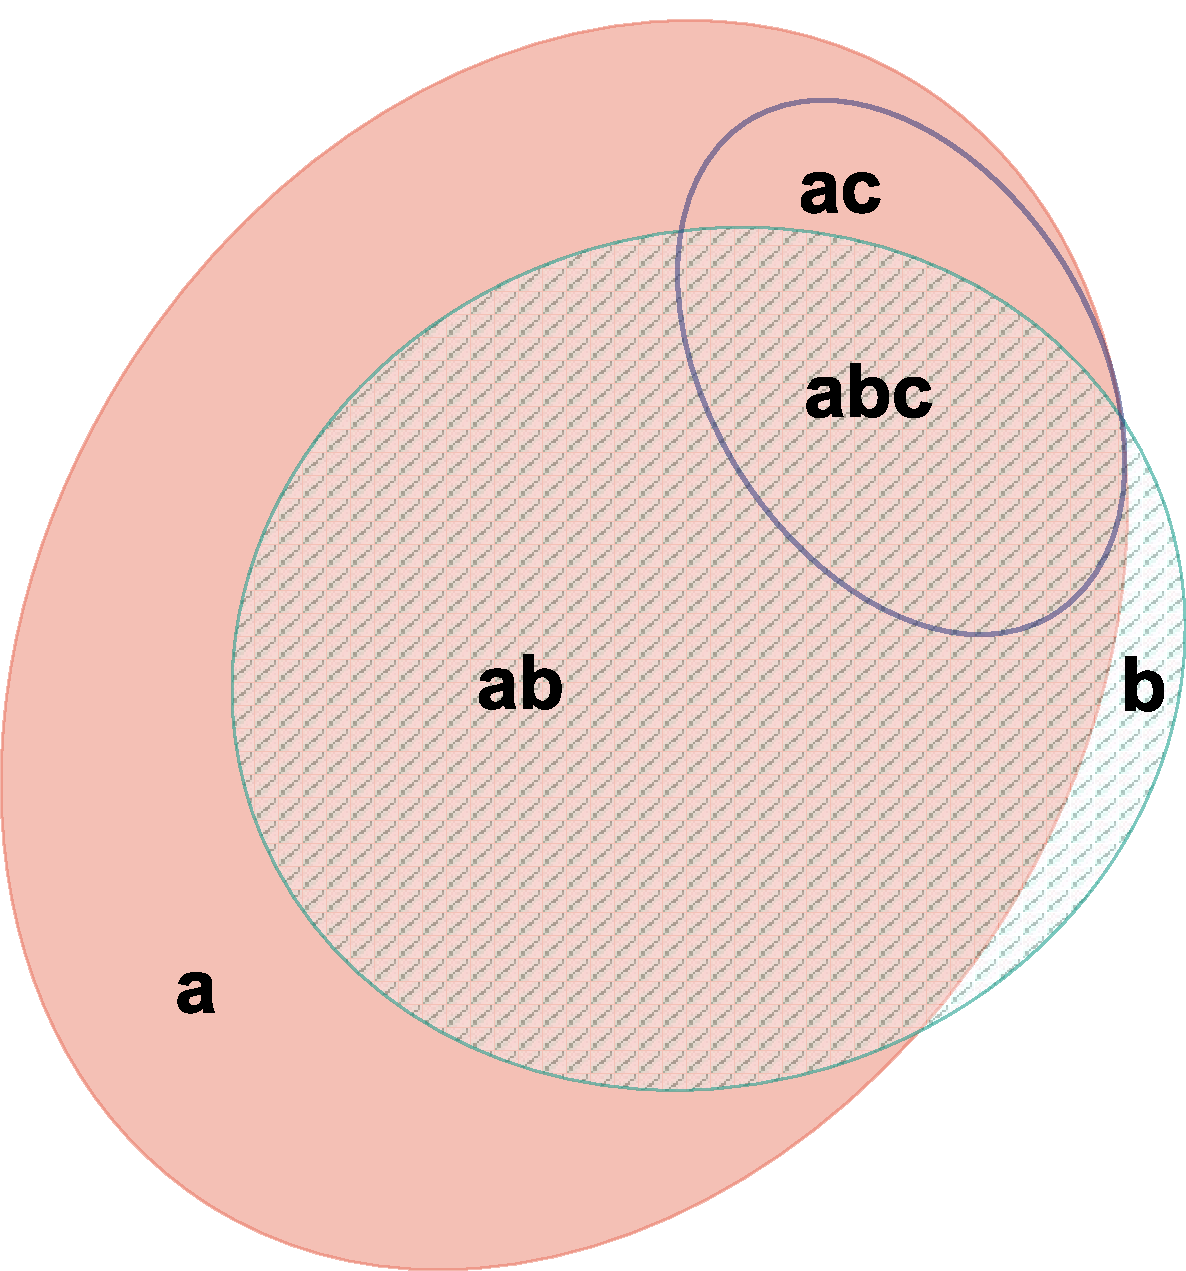
\includegraphics[height=.9\linewidth]{graphics//eulerape-lenz-a}
\subcaption{The diagram from \pkg{eulerAPE}.}
\end{subfigure}
\end{figure}

To conclude the case studies part of this thesis, we look at a diagram
that was featured on website of the author of
\pkg{venn.js}~\citep{Frederickson_2015a}, which used the
\emph{Netflix Prize Dataset}\footnote{The dataset is no longer available
on this webpage, but has been archived at
\url{https://www.kaggle.com/netflix-inc/netflix-prize-data}
for those who are interested.} from which he
\begin{quote}
[...] picked 6 movies, kind of at random -- and then represented them using the
set of users that gave the movie a 5 star rating.
\end{quote}
The movies were Amelie, Pulp Fiction, Miss Congeniality, Armageddon, Rashomon,
and Coyote Ugly. The data only includes pairwise
relationships~(\cref{tab:netflix}).

\begin{table}
\caption{The data from the Netflix Prize dataset
used in \citet{Frederickson_2015a}.\label{tab:netflix}}
\centering
\libertineTabular
\addtolength{\tabcolsep}{-2pt}
\small
\begin{tabular}{r|rrrrrr}
& \rot{Amelie} & \rot{Pulp Fiction} & \rot{Miss Congeniality} & \rot{Armageddon} & \rot{Rashomon} & \rot{Coyote Ugly}\\
\hline
Amelie            & 38,753 &&&&&\\
Pulp Fiction      & 15,197 & 70,153 &&&&\\
Miss Congeniality &  1,829 &  3,854 & 37,837 &&&\\
Armageddon        &  1,218 &  6,593 & 10,536 & 40,345 &&\\
Rashomon          &  2,087 &  2,799 &    132 &    143 & 6,209 &\\
Coyote Ugly       &    610 &  2,206 &  5,965 &  5,699 &    38 & 15,611
\end{tabular}
\end{table}



The fit from \pkg{eulerr} is marginally better than that of \pkg{venn.js}.
The stress and diagError of the \pkg{eulerr} diagram~(\cref{fig:netflix-eulerr})
are 0.003 and 0.014 respectively,
whilst the same figures are 0.004 and
0.015 for the \pkg{venn.js}
diagram~(\cref{fig:netflix-vennjs}).

\begin{figure*}[hbtp]
\begin{subfigure}[b]{.45\linewidth}
\centering
\begin{knitrout}\small
\definecolor{shadecolor}{rgb}{0.969, 0.969, 0.969}\color{fgcolor}

{\centering 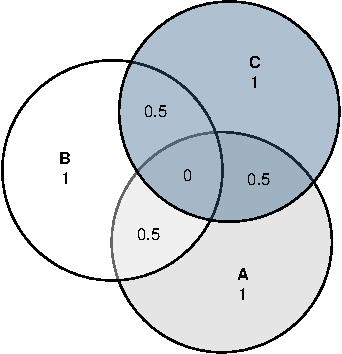
\includegraphics[width=\maxwidth]{figure/unnamed-chunk-3-1} 

}



\end{knitrout}
\subcaption{The fit from \pkg{eulerr} with a stress of
0.003 and diagError of 0.014.
\label{fig:netflix-eulerr}}
\end{subfigure}\hfill%
\begin{subfigure}[b]{.45\linewidth}
\centering
\begin{knitrout}\small
\definecolor{shadecolor}{rgb}{0.969, 0.969, 0.969}\color{fgcolor}

{\centering 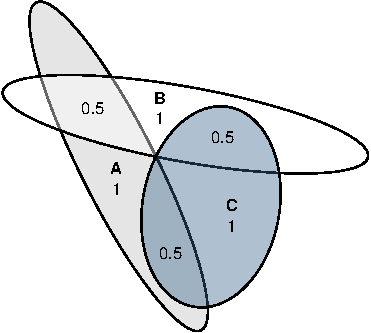
\includegraphics[width=\maxwidth]{figure/unnamed-chunk-4-1} 

}



\end{knitrout}
\subcaption{The fit from \pkg{venn.js} with a stress of
0.004 and diagError of 0.015.
\label{fig:netflix-vennjs}}
\end{subfigure}
\caption{The Euler diagrams generated from the Netflix Prize data. The
difference in the two layouts primarily concern the placements of \emph{Rashomon}
and \emph{Miss Congeniality}.}
\label{fig:netflix}
\end{figure*}

\section{Consistency}
\label{sec:consistency}

To compare the consistency among \pkg{eulerr}, \pkg{venneuler}, \pkg{eulerAPE},
\pkg{venn.js}, and \pkg{Vennerable}, we generate random diagrams of circles and
ellipses (separately), compute their areas, and attempt to reproduce the original diagrams
using the various software. We restrict ourselves to
diagrams consisting of between three and eight shapes.

For the circles, we sample radii ($r_i$) and coordinates ($h_i$ and $k_i$) from
%
\begin{equation}
\begin{aligned}
r_i     & \sim \mathcal{U}(0.2, 0.6)\\
h_i,k_i & \sim \mathcal{U}(0, 1),
\end{aligned}
\label{eq:consistencyCircles}
\end{equation}
where $N$ is the number of shapes.
For the ellipses, we sample semiaxes ($a_i$ and $b_i$), coordinates
($h_i$ and $k_i$), and rotation axes ($\phi_i$) from
%
\begin{equation}
\begin{aligned}
h_i,k_i & \sim \mathcal{U}(0, 1)\\
r_i     & \sim \mathcal{U}(0.2, 0.6)\\
c_i     & \sim \mathcal{U}(1/2, 2)\\
a_i     & = r_ic_i\\
b_i     & = r_i/c_i\\
\phi_i  & \sim \mathcal{U}(0, \pi),
\end{aligned}
\label{eq:consistencyEllipses}
\end{equation}
where $c$ is the ratio between the semiaxes.

Next, we compute the required areas, $\omega$ (from~\cref{def:omega}), for each
iteration and fit a Euler diagram using the aforementioned packages. Finally,
we compute and return \emph{diagError}~\eqref{eq:diagError} and score each
diagram as a \emph{success} if its \emph{diagError} is lower than 0.01, that is,
if no portion of the diagram is 1\% off (in absolute terms) from that of the
input; note that this is always achievable since our Euler diagrams are formed
from sampled diagrams.

For each number of shapes $(i=3,4,\dots,8)$ we run the simulations until we have
achieved a 95\% confidence interval around $\hat{p}$, the proportion of
successful diagrams, that is no wider than 2\%. The confidence that we generate
is the standard asymptotic interval,
\begin{equation*}
\mathcal{I}(\hat{p})_{0.95} = \hat{p} \pm z_{0.95}\sqrt{\frac{\hat{p}(\hat{p}-1)}{n}}
\end{equation*}
The algorithm is formalized in~\autoref{alg:consistency}. The left panel of
\cref{fig:consistency} shows the results of our simulation.

\begin{alg}
\DontPrintSemicolon
\caption{The algorithm used to simulate circles and ellipses, compute their
areas, and fit Euler diagrams to these layouts using the different software packages.\label{alg:consistency}}
\For{$i\leftarrow 3$ \KwTo $8$}{
  \While{length of each $\mathcal{I}(p_s)_{0.95} < 2\%$ \textbf{and} $j < 500$}{
    \uIf{circle}{
      $h,k    \leftarrow \mathcal{U}(0, 1)$\\
      $r      \leftarrow \mathcal{U}(0.3, 0.6)$\\
      $\omega \leftarrow \mathtt{findOverlaps}(h, k, r)$\\
    }
    \ElseIf{ellipse}{
      $h,k    \leftarrow \mathcal{U}(0, 1)$\\
      $a,b    \leftarrow \mathcal{U}(0.2, 0.8)$\\
      $\phi   \leftarrow \mathcal{U}(0, 2\pi)$\\
      $\omega \leftarrow \mathtt{findOverlaps}(h, k, a, b, \phi)$\\
    }
    $A \leftarrow \mathtt{ fitDiagram}(\omega)$\\
    $\text{diagError}_j \leftarrow \max_{k=1,2,\dots,2^i-1} \left| \frac{\omega_k}{\sum \omega_k} - \frac{A_k}{\sum A_k} \right|$\\
    \lIf{$\text{diagError}_j < 0.01$}{$\text{successes} + 1$}
    \ForEach{$s \leftarrow$ software package}{
      $\hat{p}_s \leftarrow \text{successes}/j$\\
      $\mathcal{I}(\hat{p}_s)_{0.95} \leftarrow \hat{p} \pm z_{0.95}\sqrt{\frac{\hat{p}_s(\hat{p}_s-1)}{n}}$\\
    }
  }
}
\end{alg}

\begin{figure*}[bhtp]

\begin{knitrout}\small
\definecolor{shadecolor}{rgb}{0.969, 0.969, 0.969}\color{fgcolor}

{\centering \includegraphics[width=\maxwidth]{figure/consistency-1} 

}



\end{knitrout}
\caption{Reproducibility tests for ellipses and circles generated from the
distributions from \eqref{eq:consistencyCircles}. \pkg{Vennerable}
and \pkg{eulerAPE} only accepts three-set diagrams and are hence otherwise
absent..\label{fig:consistency}}
\end{figure*}



For circular diagrams, \pkg{eulerr} outperforms \pkg{Vennerable} and \pkg{venneuler} in
consistency by considerable margin and is on par with \pkg{venn.js} and
\pkg{eulerAPE}~(\cref{fig:consistency}). \pkg{eulerr} and \pkg{eulerAPE} are
the only packages that successfully fits all of the circular diagrams (although
\pkg{eulerAPE} only accepts a subset of our three-set diagrams). \pkg{venn.js}
fails for 4 sets out of
6000 diagrams. This difference,
however, is not significant according to our asymptotic confidence interval.

For ellipses of three shapes, only \pkg{eulerr} passes the bar on each
occasion. \pkg{eulerAPE} fails in
6
cases, which again is not significantly worse.

For ellipses of four or more sets---which only \pkg{eulerr} accepts---the
consistency drops for each additional set, yet remains above
38\%. \pkg{Vennerable}, which
is only able to produce three-set diagrams, only produces accurate diagrams for
7\% of the random layouts and moreover
fails with an error in 6 cases.

\section{Accuracy}
\label{sec:accuracy}

In \nameref{sec:consistency}, we assessed the efficacy in reproducing diagrams
with exact, but unknown, solutions. Reality, however, often presents us with
relationships that lack such exact solutions. Yet, although there might not be an
exact solution, one might still exist that is \emph{good enough},
which we then want our model to find for us so that we can examine
its adequacy.

To assess the proficiency of finding approximate solutions,
we generate random set relationships that may or may not have
exact solutions and fit Euler diagram using the software under study. For each
$i=3,4,\dots,8$ sets we initialize $2^i-1$ permutations of set combinations,
select one for each set, and initialize these to a number in
$\mathcal{U}(0, 1)$. After this, we pick $0 \text{ to } \binom{N-2}{1}$ elements
from the $2^i-i-1$ remaining permutations and assign to them a number from
$\mathcal{U}(0, 1)$ as before.

As in \nameref{sec:consistency}, we run our simulations until we achieve
a 95\% confidence interval around the mean diagError no wider than 0.02,
but for a minimum of 1000 iterations. The confidence level we use is the
based on the t-distribution:
\begin{equation}
\mathcal{I}(\hat{\mu})_{0.95} = \hat{\mu} \pm t_{0.95}\frac{s}{\sqrt{n}},
\end{equation}
where $\hat{\mu} = \bar{x}$. The algorithm is formalized in~\autoref{alg:accuracy}

\begin{alg}
\DontPrintSemicolon
\caption{The algorithm we use to simulate random set relationships and fit
them with the software under study to assess their accuracy.\label{alg:accuracy}}
\For{$i\leftarrow 3$ \KwTo $8$}{
  \While{length of each $\mathcal{I}(\hat{\mu}_s)_{0.95} < 0.02$ \textbf{and} $j < 500$}{
    initialize $\omega = \{\omega_1,\omega_2,\dots,\omega_{2^i-1} \}$ to zero\\
    \For{$j\leftarrow 3$ \KwTo $i$}{
      $j \leftarrow$ random index in $\{\omega : \omega \cap F_i \neq \emptyset\}$\\
      $\omega_j \leftarrow \mathcal{U}(0, 1)$\\
    }
    $\omega_S \leftarrow \mathcal{U}\{0, i\}$ random elements from $\{\omega : \omega = 0\}$\\
    $\omega_S \leftarrow \mathcal{U}(0, 1)$\\
    fit a Euler diagram to $\omega$\\
  }
}
\end{alg}

However, given that neither \pkg{Vennerable} nor \pkg{eulerAPE} are capable
of fitting Euler diagrams that feature subset or disjoint relationships, and
because fully intersecting diagrams are more difficult to fit---at least
with circles---we run a separate treatment
in which we modify~\autoref{alg:accuracy} so that every intersection
is initialized to a value in $\mathcal{U}(\epsilon, 1)$, where
$\epsilon$ is defined as the square root of the current machine's smallest
representable difference between one and the smallest value greater than
one\footnote{The relevant line of code used to generate this tolerance is
\code{sqrt(.Machine\$double.eps)}}.



From the results generated via \autoref{alg:accuracy}, we can
surmise that elliptical \pkg{eulerr} diagrams achieve the lowest stress and
diagError on average~\cref{fig:accuracy}. It is lower regardless of the
number of sets, but is relatively more pronounced for sets of three and four shapes.

\begin{figure*}[hbtp]
\begin{knitrout}\small
\definecolor{shadecolor}{rgb}{0.969, 0.969, 0.969}\color{fgcolor}

{\centering \includegraphics[width=\maxwidth]{figure/accuracy-1} 

}



\end{knitrout}
\caption{Tukey box plots of Euler diagrams based on set relationships that may
or may not have perfect solutions, generated from~\eqref{eq:consistencyEllipses}.}
\label{fig:accuracy}
\end{figure*}

We also find that among the algorithms that fit circular Euler diagrams,
\pkg{eulerr} offers the lowest median stress across all the sizes of set
relationships. For diagError, however, \pkg{venn.js} produces diagrams with the
least loss for three sets, whilst \pkg{eulerr} scores better for all the remaining set sizes,
for which \pkg{venn.js} is moreover outdone by \pkg{venneuler}.



Looking at the results from the simulation of three-set relationships with
every intersection present~(\cref{fig:accuracy-int}), \pkg{eulerr} still
produces the most accurate diagrams (provided that we use ellipses)---both in
terms of stress and diagError. The
difference next to \pkg{eulerAPE} is very small, however, with differences
below $10^{-8}$.

\begin{figure}[hbtp]
\caption{Tukey box plots of diagError and stress for Euler diagrams
based on set relationships of three sets with every
intersection present.\label{fig:accuracy-int}}
\begin{knitrout}\small
\definecolor{shadecolor}{rgb}{0.969, 0.969, 0.969}\color{fgcolor}

{\centering \includegraphics[width=\maxwidth]{figure/accuracy-int-1} 

}



\end{knitrout}
\end{figure}

For the circular diagrams, \pkg{venn.js} achieves the lowest median diagError of
\ensuremath{7.11\times 10^{-8}} followed by \pkg{venneuler} at \ensuremath{8.219\times 10^{-7}},
\pkg{eulerr} at 0.044, \pkg{eulerAPE} at 0.035,
and \pkg{Vennerable} at 0.044. As for stress, however, the order is
partially reversed with respective stress values at
\ensuremath{4.581\times 10^{-14}}, \ensuremath{7.834\times 10^{-12}}, 0.022, 0.035,
0.044 for
\pkg{eulerr}, \pkg{venneuler}, \pkg{venn.js}, \pkg{eulerAPE}, and \pkg{Vennerable}
respectively.

\section{Performance}
\label{sec:performance}

Using the same method as in \nameref{sec:accuracy}, we generate random set
relationships and measure the time it takes for each software package to form a
diagram from the fit. We rely on \pkg{microbenchmark} for the benchmarks,
which randomizes the order in which the packages are called between trials.
Because the current version of \pkg{venn.js} has not been implemented in R, nor
any version of \pkg{eulerAPE}, we omit these packages from the
performance benchmarks.



The violin plot in \cref{fig:performance} shows that \pkg{eulerr} is speedier
for circular diagrams up to seven sets, at which point \pkg{venneuler} catches
up and then surpasses the performance of \pkg{eulerr}. For a three set diagram,
for instance, \pkg{eulerr} takes a median of
0.007
seconds to find a fit, whilst \pkg{venneuler} takes 0.414
seconds, and \pkg{Vennerable} 0.056
seconds. For eight sets, meanwhile, \pkg{eulerr} takes
2.68
seconds and \pkg{venneuler} 2.059.

The computation time for the elliptical
diagrams from \pkg{eulerr} generally vary more but are still, on average,
faster than \pkg{venneuler} for up to five sets---albeit with the exception
of diagrams of three sets, where the resulting bimodal distribution is a
consequence of the time-consuming
last-ditch optimizer (\nameref{sec:last-ditch}) that is activated by default
if the fit is not error-free.

\begin{figure*}[hbtp]
\begin{knitrout}\small
\definecolor{shadecolor}{rgb}{0.969, 0.969, 0.969}\color{fgcolor}

{\centering \includegraphics[width=\maxwidth]{figure/performance-1} 

}



\end{knitrout}
\caption{Violin plot of the performance of \pkg{eulerr}, \pkg{venneuler}, and \pkg{Vennerable} on
random set relationships of three to eight sets. The density smoother is that of \citet{Sheather_1991}.}
\label{fig:performance}
\end{figure*}

\section{Availability}\label{sec:availability}

\pkg{eulerr} is available as an R package on the CRAN network~\citep{RCT_2017a}
and is installed simply by typing

\begin{knitrout}\small
\definecolor{shadecolor}{rgb}{0.969, 0.969, 0.969}\color{fgcolor}\begin{kframe}
\begin{alltt}
\hlkwd{install.packages}\hlstd{(}\hlstr{"eulerr"}\hlstd{)}
\end{alltt}
\end{kframe}
\end{knitrout}

A development version and the source code for the project is maintained in
a GitHub repository at
\url{https://github.com/jolars/eulerr}. This version
can be installed, provided that the \pkg{devtools} package is installed,
with the following oneliner:

\begin{knitrout}\small
\definecolor{shadecolor}{rgb}{0.969, 0.969, 0.969}\color{fgcolor}\begin{kframe}
\begin{alltt}
\hlstd{devtools}\hlopt{::}\hlkwd{install_github}\hlstd{(}\hlstr{"jolars/eulerr"}\hlstd{)}
\end{alltt}
\end{kframe}
\end{knitrout}

The source code for this thesis, meanwhile, is also provided in a GitHub
repository at
\url{https://github.com/jolars/eulerrPaper},
which also hosts the code used to generate the results for this thesis is
provided.

Finally, there is a \pkg{shiny}~\citep{Chang_2017} web application for
\pkg{eulerr} at \url{http://jolars.co/eulerr}, which features
a slightly slimmed-down version that only
allows two types of input, offers less freedom in customizing the
diagram, and does not feature the last-ditch optimizer.
(See \nameref{sec:last-ditch}). The web application
s available to everyone with a internet connection and somewhat-recent web
browser.

\chapter{Discussion}
\label{ch:discussion}

In this paper, we have presented a novel method for generating Euler diagrams
for any number of sets using ellipses. We have shown that the package
performs better or on par with all the other packages for most of the analyses
in this thesis. In addition, the method is
speedier than the other R packages for set relationships with up to seven sets,
wherafter it is eclipsed by \pkg{venneuler}.

\pkg{eulerr} reproduced all the circular diagrams
generated in \nameref{sec:consistency} within our margin of error.
No other package managed this task, although the failing diagrams of both
\pkg{eulerAPE} and \pkg{venn.js} numbered in the single digits.

In contrast, \pkg{venneuler} was not (by our standards) able to adequately
reproduce between 30 and 65\%
of these  diagrams, which, however, was still better than the results on a previous
test2~\citep{Frederickson_2015b}. Some of these diagrams feature disjoint or subset
relationships, which \pkg{venneuler} have problems fitting on account of its
initial optimizer. As we discussed in the \nameref{sec:background},
\pkg{eulerr}, \pkg{venn.js}, and \pkg{venneuler} all use multi-dimensional scaling for
their initial diagram. \pkg{venneuler}, however, unnecessarily restricts the
locations of disjoint and subset circles. Given, for instance, two disjoint
sets, the algorithm will attempt to place them tangent to one another; otherwise,
the optimizer will report loss. Likewise, for a subset
relationship, \pkg{venneuler} tries to place the smaller circle at the exact
midpoint of the enclosing shape.

For the fit to be accurate, however, those restrictions are pointless as long as
the sets remain disjoint or subset and almost always feature
other locations that fulfill those requirements.
For \pkg{venneuler}, this becomes problematic when the required positions interfere
with locations of other sets that need to use that space. The
MDS algorithm from \pkg{venn.js} and \pkg{eulerr} circumvents this by
assigning a loss and gradient of zero when the pairwise set intersection
\emph{and} the candidate circles are disjoint or subset. This makes it easier
for the starting layout to find a good initial layout.

Another reason for the mediocre results of \pkg{venneuler} could be both that the optimizer
terminates prematurely in case the relative reduction in stress is considered negligible
between iterations \emph{or} that the number of iterations is generally too
low.

\pkg{eulerr} managed to also reproduce all of the elliptical
three-set diagrams perfectly but failed for a considerable portion as the number
of sets in the input surged.
For three-set diagrams, \pkg{eulerr} employs a rigorous last-ditch
optimizer in case the fit it not adequate\footnote{Here, we define \emph{adequate}
as a diagram with diagError below 0.001.} after the "final" optimization step. This step is
time-consuming (as we saw in \nameref{sec:performance}), but if activated
would yield better results also for sets of more than three shapes.

The elliptical diagrams from \pkg{eulerr} are more accuracte for random
set relationships (that might lack exact solutions) than all the
other packages in this thesis, although the elliptical diagrams from \pkg{eulerAPE}
were almost as accurate. Elliptical Euler diagrams are more successful since they,
as we briefly covered in the \nameref{sec:background},
allow two addition degrees of freedom for each set. The gain
is greatest for three sets and shrinks as we add more sets. This is what we
expect: complicated inputs require
complicated models and there are many diagrams that even elliptical Euler
diagrams cannot fit---consider, for instance, the complicated geometry of the
Venn diagram in \cref{fig:edwards} that is required to represent
all the intersections between six sets.

\begin{marginfigure}
\begin{knitrout}\small
\definecolor{shadecolor}{rgb}{0.969, 0.969, 0.969}\color{fgcolor}

{\centering \includegraphics[width=\maxwidth]{figure/battlement-1} 

}



\end{knitrout}
\caption{A six-set Venn diagram using Edward's method~\cite{Edwards_2014};
this diagram was generated with \pkg{Vennerable}.}
\label{fig:edwards}
\end{marginfigure}

Considering only circular Euler diagrams, \pkg{eulerr} remains the best
choice for both diagError and stress in all cases except for three-set
diagrams, where it ranks best in terms of stress but not diagError\footnote{
It might be appropriate to note that \pkg{eulerr} and \pkg{venn.js} both
attempt to minimize the sums of squares and not diagError.}; \pkg{venn.js}
scores lowest. Interestingly---as well as surprisingly, given the results
from \nameref{sec:consistency}---\pkg{venn.js} performs worse than \pkg{venneuler}
in all of the remaining cases. We can only speculate as to reasons for this,
but it possible that the Nelder--Mead variant that was written for \pkg{venn.js}
has trouble finding a good fit; indeed, this was our experience when designing
\pkg{eulerr}, which at one point featured a variety of the same optimizer; in our case,
\code{nlm()} from R, which uses numerical derivatives, was
found to be superior.

For three to seven sets, \pkg{eulerr} is faster than both \pkg{Vennerable} and
\pkg{venneuler}. The reason for this is partly the implementation
in C++ and the use of the Armadillo library~\citep{Sanderson_2016} provided by the interfaces
\pkg{Rcpp}~\citep{Eddelbuettel_2011} and \pkg{RcppArmadillo}~\citep{Eddelbuettel_2014}.
The second reason is the exact-area computations that outperform the
quadtree binning of \pkg{venneuler} for the lower amount of sets.
Paradoxically, this is also why the performance of \pkg{eulerr}
suffers as the number of sets increase beyond seven.

The bottleneck in \pkg{eulerr}'s performance is the final
optimization. It has to examine every possible intersection when computing the
areas. For eight sets, for instance, this means investigating $255$
intersections. In theory, the
algorithm should converge in $\mathcal{O}(2^n)$ time. \citet{Wilkinson_2012},
meanwhile, report convergence in $\mathcal{O}(n)$ time. There is evidence
of this in \cref{fig:performance} and it is possible that a fine-tuned
version of \pkg{venneuler}'s algorithm might outperform \pkg{eulerr} also
for lower number of sets. Regardless, the increasing computational demand
of large number of sets make fitting such diagrams prohibitive at least in
exploratory data analysis. Although it is questionable whether there is much
use for Euler diagrams for such complicated diagrams---only rarely willl they
surrender to an adequate fit---future versions of this algorithm should
consider implementing approximate area-calculations when the number of sets is
large.

Fitting diagrams is substantially harder with ellipses than with circles.
There are many more local minimi that might hobble our optimizer
and since our initial configuration only
considers circles, such minimi cannot reliably be avoided before the final
optimization step. And because we moreover default to a semi-local optimizer in this final step,
it is not uncommon that we become stuck before finding the global minimum.
The last-ditch optimizer
battles such minimi with brute force: it tries a considerable number of permutations
and uses the previous fits (initial and semi-final) only to set up
constraints for the algorithm. The downside to using this optimizer is that it,
in contrast to us, people\footnote{And the other
optimizer that begins with an initial layout of circles.},
does not prefer circles over ellipses, which means that we might get diagrams
with ellipses when circles would do just as well.

\section{Conclusion}
\label{sec:conclusion}

In the majority of scenarios examined in this thesis,
\pkg{eulerr} offers solutions with the least error among all of the packages
tested. For three sets, its performance is equalled by the elliptical diagrams that
\pkg{eulerAPE} produce, which, however, impose the restrictions that
\pkg{eulerr} do not, namely, that there be no disjoint or subset relationships.
In addition, \pkg{eulerr} offers considerable control over the visual output,
which is levied via the \pkg{lattice} package for R.

\pkg{eulerAPE}'s restriction to three sets is discussed by the authors of the
package, who motivate this limitation with the propensity of Euler diagrams with
more sets to lack adequate solutions and that their complexity make
implementations difficult~\citep{Micallef_2013}. Whilst it is true that
inputs with more than three sets do not always reduce to adequate Euler diagrams,
it is our stance that those that do warrant a software implementation that
can help the user find them, given that Euler diagrams are intuitive
graphics that are appreciated by most viewers.

The primary shortcoming of \pkg{eulerr} lies in its failure to consistently
reproduce random elliptical diagrams (see \nameref{sec:consistency}), implying that the
performance in producing random set relationships (see \nameref{sec:accuracy})
must have potential to improve. This is not an intractable problem and we
argue that it can be overcome either by
\begin{itemize}
\item relying on brute force global optimizers that thoroughly examine
the search space and attempt to optimize, and possibly parallelize,
these to make larger diagrams fit within a reasonable time span, or
\item designing an algorithm for the initial configuration that works specifically for
ellipses.
\end{itemize}
Whichever direction future algorithms take, we believe that the advances
presented in this thesis should serve as another step forward towards more
accurate Euler diagrams.

\section{Acknowledgements}
\label{sec:acknowledgements}

Thanks to blabla.

\begin{fullwidth}
\part*{Appendices}
\end{fullwidth}
\appendix
\chapter{Visualization}
\label{ap:visualization}

Once we have ascertained that our Euler diagram fits well, we can turn to
visualizing the solution. For this purpose, \pkg{eulerr} leverages the
\pkg{Lattice} graphics system~\citep{Sarkar_2008} for R to offer intuitive and
granular control over the output.

Plotting the ellipses is straightforward using the parametrization of a rotated
ellipse,
%
\begin{equation*}
\begin{bmatrix}
  x \\ y
\end{bmatrix} =
\begin{bmatrix}
  h + a \cos{\theta} \\
  k + b \sin{\theta}
\end{bmatrix},\quad \text{where } \theta \in [0, 2\pi].
\end{equation*}
%
Often, however, we would also like to label the ellipses and their intersections
with text and this is considerably more involved.

\section{Labeling}
\label{sec:labeling}

Labeling the ellipses is difficult because the shapes of the intersections
often are irregular, lacking a well-defined center; we know of no analytical
solution to this problem. As usual, however, the next-best option turns out to
be a numerical one. First, we locate a point that is inside the required region
by spreading points across the discs involved in the set intersection. To
distribute the points, we use a modification of
\emph{Vogel's method}~\citep{Arthur_2015,Vogel_1979} adapted to ellipses.
Vogel's method spreads points across a disc using
\begin{equation}
p_k =
\begin{bmatrix}
  \rho_k \\
  \theta_k
\end{bmatrix} =
\begin{bmatrix}
  r \sqrt{\frac{k}{n}}\\
  \pi (3 - \sqrt{5})(k - 1)
\end{bmatrix}\quad\text{for } k = 1, 2,\dots, n.
\label{eq:vogel}
\end{equation}
In our modification, we scale, rotate, and translate the points formed
in~\eqref{eq:vogel} to match the candidate ellipse. We rely, as before, on
projective geometry to carry out the transformations in one go:
\[
p' =
\begin{bmatrix}
  x' \\
  y' \\
  1
\end{bmatrix} =
\begin{bmatrix}
  1 & 0 & h \\
  0 & 1 & k \\
  0 & 0 & 1
\end{bmatrix}
\begin{bmatrix}
  \cos{\phi}  & \sin{\phi} & 0 \\
  -\sin{\phi} & \cos{\phi} & 0\\
  0           & 0          & 1
\end{bmatrix}
\begin{bmatrix}
  a & 0 & 0 \\
  0 & b & 0 \\
  0 & 0 & 1
\end{bmatrix}
\begin{bmatrix}
  \hat{x} \\
  \hat{y} \\
  1
\end{bmatrix}
\]
After we spread our points throughout the ellipse and find a point, $p'_i$, that
is contained in our desired intersection, we proceed to optimize its position
numerically. The position we are looking for is that which maximizes the
distance to the closest ellipse in our diagram to provide as much margin as
possible for the label. This is a maximin problem with a loss function equal to
\begin{equation}
\max_{x,y \in \mathbb{R}^2} \min_{i=1,2,\dots,N} f(x,y,h_i,k_i,a_i,b_i,\phi_i)
\label{eq:lossDist}
\end{equation}
where $f$ is the function that determines the distance from a point ($x,y$) to the ellipse defined by $h,k,a,b$ and $\phi$.

Similarly to fitting Euler diagrams in the general case, there appears to be no
analytical solution to computing the distance from a point to an ellipse. The
numerical solution we use has been described in~\citet{Eberly_2016a} and
involves solving the roots to a quartic polynomial via a robust
bisection optimizer.

To optimize the location of the label, we employ a version of the
\emph{Nelder--Mead Method}~\citep{Nelder_1965} which has been translated from
\citet{Kelley_1999} and adapted for \pkg{eulerr} to ensure that is coverges
quickly and that the simplex remains within the intersection boundaries
(since we want the local maximum). The method is visualized in~\cref{fig:vogel}.
\begin{marginfigure}
\begin{knitrout}\small
\definecolor{shadecolor}{rgb}{0.969, 0.969, 0.969}\color{fgcolor}

{\centering \includegraphics[width=\maxwidth]{figure/vogel-1} 
\includegraphics[width=\maxwidth]{figure/vogel-2} 
\includegraphics[width=\maxwidth]{figure/vogel-3} 

}



\end{knitrout}
\caption{The method eulerr uses to locate an optimal position for a label in
three steps from top to bottom: first, we spread sample points on one of the
ellipses and pick one inside the intersection of interest, then we begin moving
it numerically, and finally place our label.}
\label{fig:vogel}
\end{marginfigure}

\section{Aesthetics}
\label{sec:aesthetics}

Euler diagrams display both quantitative and qualitative data. The quantitative
aspect is the quantities or sizes of the sets depicted in the diagram and is
visualized by the relative sizes, and possibly the labels, of the areas of the
shapes---this is the main focus of this paper. The qualitative aspects,
meanwhile, consist of the mapping of each set to some quality or category, such
as having a certain gene or not. In the diagram, these qualities can be
separated through any of the following aesthetics:
%
\begin{itemize}
\item color,
\item border type,
\item text labelling,
\item transperancy,
\item patterns,
\end{itemize}
%
or a combination of these. The main purpose of these aethetics is to separate
out the different ellipses so that the audience may interpret the diagram with
ease and clarity.

Among these aesthetics, the best choice (from a viewer perspective) appears to
be color~\citep{Blake_2016}, which provides useful information without
extraneous chart junk~\citep{Tufte_2001}. The issue with color, however, is that
it cannot be perceived perfectly by all---8\% of men and 0.4\% of women in
European Caucasian countries, for instance, suffer the most common form,
red--green color deficiency~\cite{Birch_2012}. Moreover, color
is often printed at a premium in scientific publications and adds no information
to a diagram of two shapes.

For these reasons, \pkg{eulerr} defaults to distinguishing ellipses with color
using a color palette generated via the R package
\pkg{qualpalr}~\citep{Larsson_2016}, which automatically generates qualitative
color palettes based on a perceptual model of color vision that optionally
caters to color vision deficiency. This palette has been manually modified
to fullfil our other objectives of avoiding using colors for two
sets. The first eight colors of the pallete are visualized in
\cref{fig:colorexample}.

\begin{figure}[htbp]
\caption{The eight first colors of the default color palette.\label{fig:colorexample}}
\begin{knitrout}\small
\definecolor{shadecolor}{rgb}{0.969, 0.969, 0.969}\color{fgcolor}

{\centering \includegraphics[width=\maxwidth]{figure/colorexamle-1} 

}



\end{knitrout}
\end{figure}

\section{Normalizing dispered layouts}
\label{sec:layout}

If there are disjoint clusters of ellipses, the optimizer will often
spread these out more than is necessary, wasting space in our diagram. To
tackle this, we
use a SKYLINE-BL rectangle packing algorithm~\citep{Jylaenki_2010}
designed specifically for \pkg{eulerr}. In it, we surround each ellipse cluster
with a bounding box, pack these boxes into a bin of appropriate size and
aspect ratio, and adjust the coordinates of the ellipses in the clusters to
compact our diagram.

As a bonus, this also increases the chance of having
similar layouts for different function calls even when we do not
fix the random seed.

\chapter{Usage}\label{ch:usage}

\code{euler()} and \code{plot()} are the only functions that a user of
\pkg{eulerr} need concern themselves with. In \nameref{sec:input}, we described
the various forms of input that the function can be supplied with. Using the
first form, we will showcases how a Euler diagram is fit. For this example,
we use a diagram from a publication by \citet{Junta_2009} that was also
showcased in \citet{Wilkinson_2012}. We load the package,
specify our diagram, and fit it using \code{euler()} as follows.

\begin{knitrout}\small
\definecolor{shadecolor}{rgb}{0.969, 0.969, 0.969}\color{fgcolor}\begin{kframe}
\begin{alltt}
\hlkwd{library}\hlstd{(eulerr)}
\hlstd{junta_2009} \hlkwb{<-} \hlkwd{c}\hlstd{(}\hlstr{"SE"} \hlstd{=} \hlnum{13}\hlstd{,} \hlstr{"Treat"} \hlstd{=} \hlnum{28}\hlstd{,} \hlstr{"Anti-CCP"} \hlstd{=} \hlnum{101}\hlstd{,}
                \hlstr{"DAS28"} \hlstd{=} \hlnum{91}\hlstd{,} \hlstr{"SE&Treat"} \hlstd{=} \hlnum{1}\hlstd{,} \hlstr{"SE&DAS28"} \hlstd{=} \hlnum{14}\hlstd{,}
                \hlstr{"Treat&Anti-CCP"} \hlstd{=} \hlnum{6}\hlstd{,} \hlstr{"SE&Anti-CCP&DAS28"} \hlstd{=} \hlnum{1}\hlstd{)}
\hlstd{fit1} \hlkwb{<-} \hlkwd{euler}\hlstd{(junta_2009)}
\end{alltt}
\end{kframe}
\end{knitrout}

Printing the results provides a summary of the fit, including the \emph{stress}
and \emph{diagError} metrics that were introduced in~\nameref{sec:gof}.

\begin{knitrout}\small
\definecolor{shadecolor}{rgb}{0.969, 0.969, 0.969}\color{fgcolor}\begin{kframe}
\begin{alltt}
\hlstd{fit1} \hlcom{# or equivalently print(fit1)}
\end{alltt}
\begin{verbatim}
##                         original fitted residuals regionError
## SE                            13 12.780     0.220       0.000
## Treat                         28 27.525     0.475       0.000
## Anti-CCP                     101 99.287     1.713       0.002
## DAS28                         91 89.457     1.543       0.001
## SE&Treat                       1  0.983     0.017       0.000
## SE&Anti-CCP                    0  0.000     0.000       0.000
## SE&DAS28                      14 13.763     0.237       0.000
## Treat&Anti-CCP                 6  5.898     0.102       0.000
## Treat&DAS28                    0  0.000     0.000       0.000
## Anti-CCP&DAS28                 0  0.000     0.000       0.000
## SE&Treat&Anti-CCP              0  0.000     0.000       0.000
## SE&Treat&DAS28                 0  0.000     0.000       0.000
## SE&Anti-CCP&DAS28              1  0.000     1.000       0.004
## Treat&Anti-CCP&DAS28           0  0.000     0.000       0.000
## SE&Treat&Anti-CCP&DAS28        0  0.000     0.000       0.000
## 
## diagError: 0.004 
## stress:    0
\end{verbatim}
\end{kframe}
\end{knitrout}

The fit is more or less equivalent to that of
\pkg{venneuler}~\citep{Wilkinson_2012}. There \emph{is} an error but it is
small at a diagError of 0.004. We could, however, try to
improve the fit using ellipses:

\begin{knitrout}\small
\definecolor{shadecolor}{rgb}{0.969, 0.969, 0.969}\color{fgcolor}\begin{kframe}
\begin{alltt}
\hlcom{# Fit the data using ellipses instead}
\hlstd{fit2} \hlkwb{<-} \hlkwd{euler}\hlstd{(junta_2009,} \hlkwc{shape} \hlstd{=} \hlstr{"ellipse"}\hlstd{)}

\hlcom{# Compare the fits on diagerror}
\hlstd{fit1}\hlopt{$}\hlstd{diagError} \hlopt{-} \hlstd{fit2}\hlopt{$}\hlstd{diagError}
\end{alltt}
\begin{verbatim}
## [1] 0
\end{verbatim}
\end{kframe}
\end{knitrout}

Comparing the two fits in diagError, however, shows that we have not bettered
the fit in any meaningful way. Our next goal is to visualize the layout, which
we do both using the default options and by customizing the fit, adding
quantities, replacing the sets' labels with a key, removing lines, and changing the
fills using the \pkg{RColorBrewer} package~(\cref{fig:plotting}).

\begin{knitrout}\small
\definecolor{shadecolor}{rgb}{0.969, 0.969, 0.969}\color{fgcolor}\begin{kframe}
\begin{alltt}
\hlstd{p1} \hlkwb{<-} \hlkwd{plot}\hlstd{(fit1)}
\hlstd{p2} \hlkwb{<-} \hlkwd{plot}\hlstd{(fit1,}
           \hlkwc{quantities} \hlstd{=} \hlkwd{list}\hlstd{(}\hlkwc{fontface} \hlstd{=} \hlnum{3}\hlstd{),}
           \hlkwc{fill} \hlstd{= RColorBrewer}\hlopt{::}\hlkwd{brewer.pal}\hlstd{(}\hlnum{4}\hlstd{,} \hlstr{"Set2"}\hlstd{),}
           \hlkwc{border} \hlstd{=} \hlstr{"transparent"}\hlstd{,}
           \hlkwc{auto.key} \hlstd{=} \hlkwd{list}\hlstd{(}\hlkwc{space} \hlstd{=} \hlstr{"right"}\hlstd{))} \hlcom{# key on the right}
\end{alltt}
\end{kframe}
\end{knitrout}

\begin{figure}[hbtp]
\caption{The same fit visualized in two distinct ways.\label{fig:plotting}}
\begin{subfigure}[b]{.4\linewidth}
\begin{knitrout}\small
\definecolor{shadecolor}{rgb}{0.969, 0.969, 0.969}\color{fgcolor}

{\centering \includegraphics[width=\maxwidth]{figure/twofits1-1} 

}



\end{knitrout}
\subcaption{The default settings.}
\end{subfigure}%
\begin{subfigure}[b]{.6\linewidth}
\begin{knitrout}\small
\definecolor{shadecolor}{rgb}{0.969, 0.969, 0.969}\color{fgcolor}

{\centering \includegraphics[width=\maxwidth]{figure/twofits2-1} 

}



\end{knitrout}
\subcaption{Custom plot settings.}
\end{subfigure}
\end{figure}

\begin{fullwidth}
\bibliography{eulerr}
\bibliographystyle{unsrtnat}
\end{fullwidth}

\end{document}
